% Created by tikzDevice version 0.12.3.1 on 2022-09-02 10:49:13
% !TEX encoding = UTF-8 Unicode
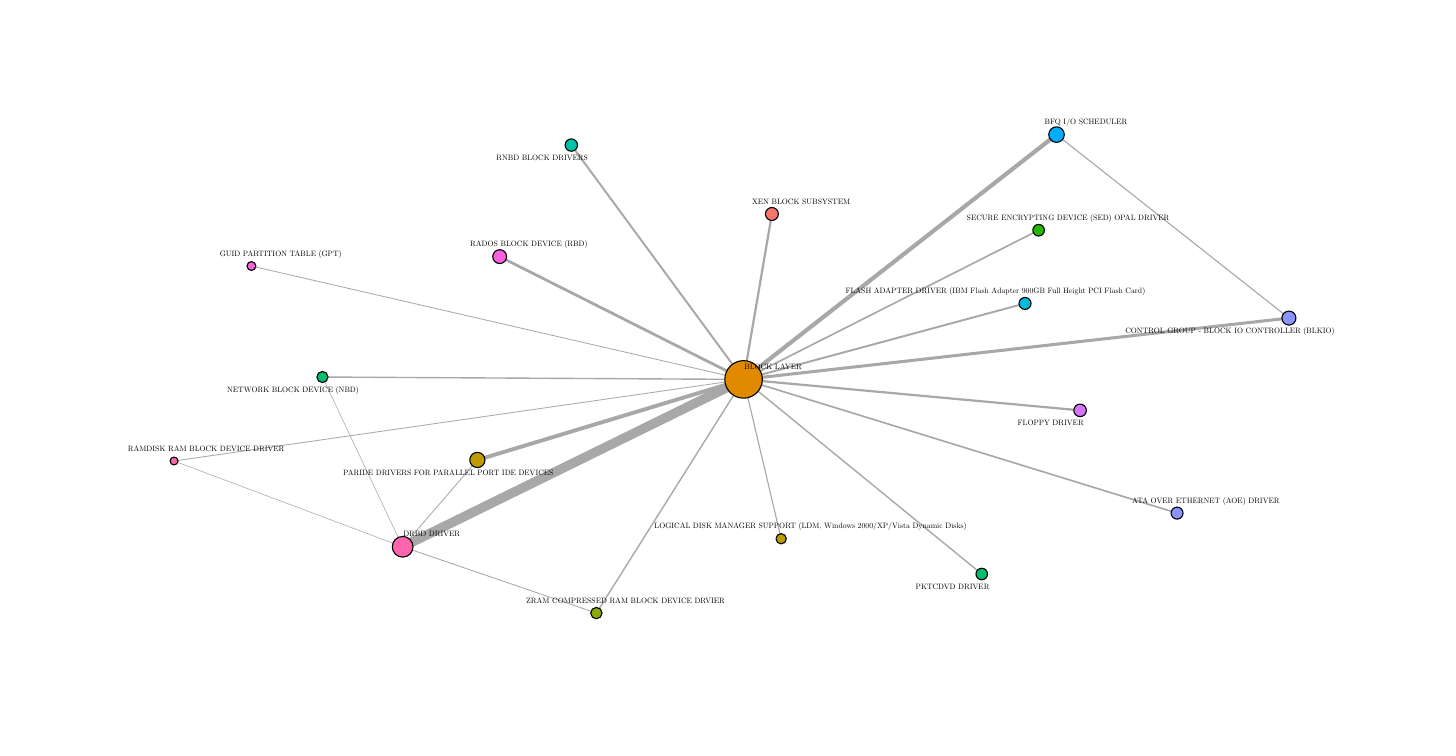
\begin{tikzpicture}[x=1pt,y=1pt]
\definecolor{fillColor}{RGB}{255,255,255}
\path[use as bounding box,fill=fillColor,fill opacity=0.00] (0,0) rectangle (505.89,252.94);
\begin{scope}
\path[clip] (  0.00,  0.00) rectangle (505.89,252.94);
\definecolor{fillColor}{RGB}{255,255,255}

\path[fill=fillColor] (  0.00,  0.00) rectangle (505.89,252.94);
\end{scope}
\begin{scope}
\path[clip] ( 32.75, 32.75) rectangle (475.89,222.94);
\definecolor{drawColor}{gray}{0.66}

\path[draw=drawColor,line width= 0.6pt,line join=round] (415.33, 77.53) -- (258.69,125.84);

\path[draw=drawColor,line width= 1.5pt,line join=round] (371.77,214.30) -- (258.69,125.84);

\path[draw=drawColor,line width= 0.4pt,line join=round] (371.77,214.30) -- (455.75,148.00);

\path[draw=drawColor,line width= 1.1pt,line join=round] (258.69,125.84) -- (455.75,148.00);

\path[draw=drawColor,line width= 3.4pt,line join=round] (258.69,125.84) -- (135.50, 65.36);

\path[draw=drawColor,line width= 0.7pt,line join=round] (258.69,125.84) -- (360.39,153.29);

\path[draw=drawColor,line width= 0.8pt,line join=round] (258.69,125.84) -- (380.29,114.66);

\path[draw=drawColor,line width= 0.3pt,line join=round] (258.69,125.84) -- ( 80.85,166.81);

\path[draw=drawColor,line width= 0.4pt,line join=round] (258.69,125.84) -- (272.27, 68.26);

\path[draw=drawColor,line width= 0.5pt,line join=round] (258.69,125.84) -- (106.51,126.70);

\path[draw=drawColor,line width= 1.4pt,line join=round] (258.69,125.84) -- (162.50, 96.73);

\path[draw=drawColor,line width= 0.5pt,line join=round] (258.69,125.84) -- (344.75, 55.52);

\path[draw=drawColor,line width= 1.0pt,line join=round] (258.69,125.84) -- (170.56,170.21);

\path[draw=drawColor,line width= 0.3pt,line join=round] (258.69,125.84) -- ( 52.89, 96.36);

\path[draw=drawColor,line width= 0.7pt,line join=round] (258.69,125.84) -- (196.44,210.52);

\path[draw=drawColor,line width= 0.6pt,line join=round] (258.69,125.84) -- (365.30,179.75);

\path[draw=drawColor,line width= 0.8pt,line join=round] (258.69,125.84) -- (268.92,185.61);

\path[draw=drawColor,line width= 0.5pt,line join=round] (258.69,125.84) -- (205.50, 41.40);

\path[draw=drawColor,line width= 0.2pt,line join=round] (135.50, 65.36) -- (106.51,126.70);

\path[draw=drawColor,line width= 0.3pt,line join=round] (135.50, 65.36) -- (162.50, 96.73);

\path[draw=drawColor,line width= 0.2pt,line join=round] (135.50, 65.36) -- ( 52.89, 96.36);

\path[draw=drawColor,line width= 0.3pt,line join=round] (135.50, 65.36) -- (205.50, 41.40);
\definecolor{drawColor}{RGB}{0,0,0}
\definecolor{fillColor}{RGB}{139,147,255}

\path[draw=drawColor,line width= 0.4pt,line join=round,line cap=round,fill=fillColor] (415.33, 77.53) circle (  2.16);
\definecolor{fillColor}{RGB}{0,172,252}

\path[draw=drawColor,line width= 0.4pt,line join=round,line cap=round,fill=fillColor] (371.77,214.30) circle (  2.81);
\definecolor{fillColor}{RGB}{225,138,0}

\path[draw=drawColor,line width= 0.4pt,line join=round,line cap=round,fill=fillColor] (258.69,125.84) circle (  6.78);
\definecolor{fillColor}{RGB}{139,147,255}

\path[draw=drawColor,line width= 0.4pt,line join=round,line cap=round,fill=fillColor] (455.75,148.00) circle (  2.53);
\definecolor{fillColor}{RGB}{255,101,172}

\path[draw=drawColor,line width= 0.4pt,line join=round,line cap=round,fill=fillColor] (135.50, 65.36) circle (  3.74);
\definecolor{fillColor}{RGB}{0,187,218}

\path[draw=drawColor,line width= 0.4pt,line join=round,line cap=round,fill=fillColor] (360.39,153.29) circle (  2.17);
\definecolor{fillColor}{RGB}{213,117,254}

\path[draw=drawColor,line width= 0.4pt,line join=round,line cap=round,fill=fillColor] (380.29,114.66) circle (  2.27);
\definecolor{fillColor}{RGB}{249,98,221}

\path[draw=drawColor,line width= 0.4pt,line join=round,line cap=round,fill=fillColor] ( 80.85,166.81) circle (  1.60);
\definecolor{fillColor}{RGB}{190,156,0}

\path[draw=drawColor,line width= 0.4pt,line join=round,line cap=round,fill=fillColor] (272.27, 68.26) circle (  1.86);
\definecolor{fillColor}{RGB}{0,190,112}

\path[draw=drawColor,line width= 0.4pt,line join=round,line cap=round,fill=fillColor] (106.51,126.70) circle (  2.01);
\definecolor{fillColor}{RGB}{190,156,0}

\path[draw=drawColor,line width= 0.4pt,line join=round,line cap=round,fill=fillColor] (162.50, 96.73) circle (  2.75);
\definecolor{fillColor}{RGB}{0,190,112}

\path[draw=drawColor,line width= 0.4pt,line join=round,line cap=round,fill=fillColor] (344.75, 55.52) circle (  2.08);
\definecolor{fillColor}{RGB}{249,98,221}

\path[draw=drawColor,line width= 0.4pt,line join=round,line cap=round,fill=fillColor] (170.56,170.21) circle (  2.50);
\definecolor{fillColor}{RGB}{255,101,172}

\path[draw=drawColor,line width= 0.4pt,line join=round,line cap=round,fill=fillColor] ( 52.89, 96.36) circle (  1.43);
\definecolor{fillColor}{RGB}{0,193,171}

\path[draw=drawColor,line width= 0.4pt,line join=round,line cap=round,fill=fillColor] (196.44,210.52) circle (  2.23);
\definecolor{fillColor}{RGB}{36,183,0}

\path[draw=drawColor,line width= 0.4pt,line join=round,line cap=round,fill=fillColor] (365.30,179.75) circle (  2.09);
\definecolor{fillColor}{RGB}{248,118,109}

\path[draw=drawColor,line width= 0.4pt,line join=round,line cap=round,fill=fillColor] (268.92,185.61) circle (  2.34);
\definecolor{fillColor}{RGB}{140,171,0}

\path[draw=drawColor,line width= 0.4pt,line join=round,line cap=round,fill=fillColor] (205.50, 41.40) circle (  2.05);

\node[text=drawColor,anchor=base,inner sep=0pt, outer sep=0pt, scale=  0.28] at (425.75, 81.06) {ATA OVER ETHERNET (AOE) DRIVER};

\node[text=drawColor,anchor=base,inner sep=0pt, outer sep=0pt, scale=  0.28] at (382.40,217.89) {BFQ I/O SCHEDULER};

\node[text=drawColor,anchor=base,inner sep=0pt, outer sep=0pt, scale=  0.28] at (269.35,129.40) {BLOCK LAYER};

\node[text=drawColor,anchor=base,inner sep=0pt, outer sep=0pt, scale=  0.28] at (434.45,142.50) {CONTROL GROUP - BLOCK IO CONTROLLER (BLKIO)};

\node[text=drawColor,anchor=base,inner sep=0pt, outer sep=0pt, scale=  0.28] at (145.99, 68.91) {DRBD DRIVER};

\node[text=drawColor,anchor=base,inner sep=0pt, outer sep=0pt, scale=  0.28] at (349.69,156.91) {FLASH ADAPTER DRIVER (IBM Flash Adapter 900GB Full Height PCI Flash Card)};

\node[text=drawColor,anchor=base,inner sep=0pt, outer sep=0pt, scale=  0.28] at (369.66,109.12) {FLOPPY DRIVER};

\node[text=drawColor,anchor=base,inner sep=0pt, outer sep=0pt, scale=  0.28] at ( 91.43,170.40) {GUID PARTITION TABLE (GPT)};

\node[text=drawColor,anchor=base,inner sep=0pt, outer sep=0pt, scale=  0.28] at (282.89, 71.81) {LOGICAL DISK MANAGER SUPPORT (LDM, Windows 2000/XP/Vista Dynamic Disks)};

\node[text=drawColor,anchor=base,inner sep=0pt, outer sep=0pt, scale=  0.28] at ( 95.88,121.20) {NETWORK BLOCK DEVICE (NBD)};

\node[text=drawColor,anchor=base,inner sep=0pt, outer sep=0pt, scale=  0.28] at (152.00, 91.22) {PARIDE DRIVERS FOR PARALLEL PORT IDE DEVICES};

\node[text=drawColor,anchor=base,inner sep=0pt, outer sep=0pt, scale=  0.28] at (334.22, 50.01) {PKTCDVD DRIVER};

\node[text=drawColor,anchor=base,inner sep=0pt, outer sep=0pt, scale=  0.28] at (181.11,173.79) {RADOS BLOCK DEVICE (RBD)};

\node[text=drawColor,anchor=base,inner sep=0pt, outer sep=0pt, scale=  0.28] at ( 64.48, 99.90) {RAMDISK RAM BLOCK DEVICE DRIVER};

\node[text=drawColor,anchor=base,inner sep=0pt, outer sep=0pt, scale=  0.28] at (185.89,205.02) {RNBD BLOCK DRIVERS};

\node[text=drawColor,anchor=base,inner sep=0pt, outer sep=0pt, scale=  0.28] at (375.95,183.29) {SECURE ENCRYPTING DEVICE (SED) OPAL DRIVER};

\node[text=drawColor,anchor=base,inner sep=0pt, outer sep=0pt, scale=  0.28] at (279.50,189.15) {XEN BLOCK SUBSYSTEM};

\node[text=drawColor,anchor=base,inner sep=0pt, outer sep=0pt, scale=  0.28] at (216.05, 44.94) {ZRAM COMPRESSED RAM BLOCK DEVICE DRVIER};
\end{scope}
\end{tikzpicture}
